\documentclass[a4paper,11pt]{article}
\usepackage[utf8]{inputenc}
\usepackage{amssymb}
\usepackage{amsmath} 
\usepackage{enumerate}
\usepackage{graphicx}
\usepackage[font=small,labelfont=bf]{caption}
\graphicspath{ {./img/} }
\DeclareMathOperator*{\argmax}{arg\!\max}
\DeclareMathOperator*{\argmin}{arg\!\min}
\DeclareMathOperator*{\Ga}{Ga}
\DeclareMathOperator*{\var}{var}
\newcounter{exercise}
\setcounter{exercise}{0}
\newcounter{subexercise}
\newcommand*{\exercise}[1][]{
  \subsection*{Exercise
    \ifx/#1/\stepcounter{exercise}\arabic{exercise}
    \else#1\fi
  }
  \setcounter{subexercise}{0}
}
\newcommand*{\subexercise}[1][]{
  \par{
    \noindent\textbf{\ifx/#1/\protect\stepcounter{subexercise}\alph{subexercise}\else#1\fi.\quad}
  }
}
\title{Chapter 23}
\author{stevenjin8}
\date{July 18, 2021}

\begin{document}
	\maketitle

	\section*{Comments and Proofs}
	Another way to think of importance sampling is that we are trying to estimate $p$, but some
	regions of $p$ are more important than others (e.g. when $f \dot p$ is large for equation 23.19).
	Thus sampling from $q$ lets us estimate $p$, but with a high resolution in regions that are more
	important

	Initially, I thought that it would be best to sample from
	regions where $\lvert \frac{ d }{ d \mathbf{x} } f( \mathbf{x} )p( \mathbf{x} )$, since those are the
	regions points aren't representative of their neighbours. But then I realized that if the Hessian
	of $f \dot p$ is small, then $f( \mathbf{x} )p( \mathbf{x} )$ will be representative of its
	neighbourhood, despite not being necessarily representative of its neighbours. In that case, it
	might be best case to sample from regions where
	$\left\lvert \frac{ d^2 }{ d \mathbf{x} \mathbf{dx}^T } f( \mathbf{x} )p( \mathbf{x} ) \right\rvert$
	might also be better.

	\section*{Exercises}
	\setcounter{exercise}{1}
	\exercise
	\begin{figure}[t]
	\centering
	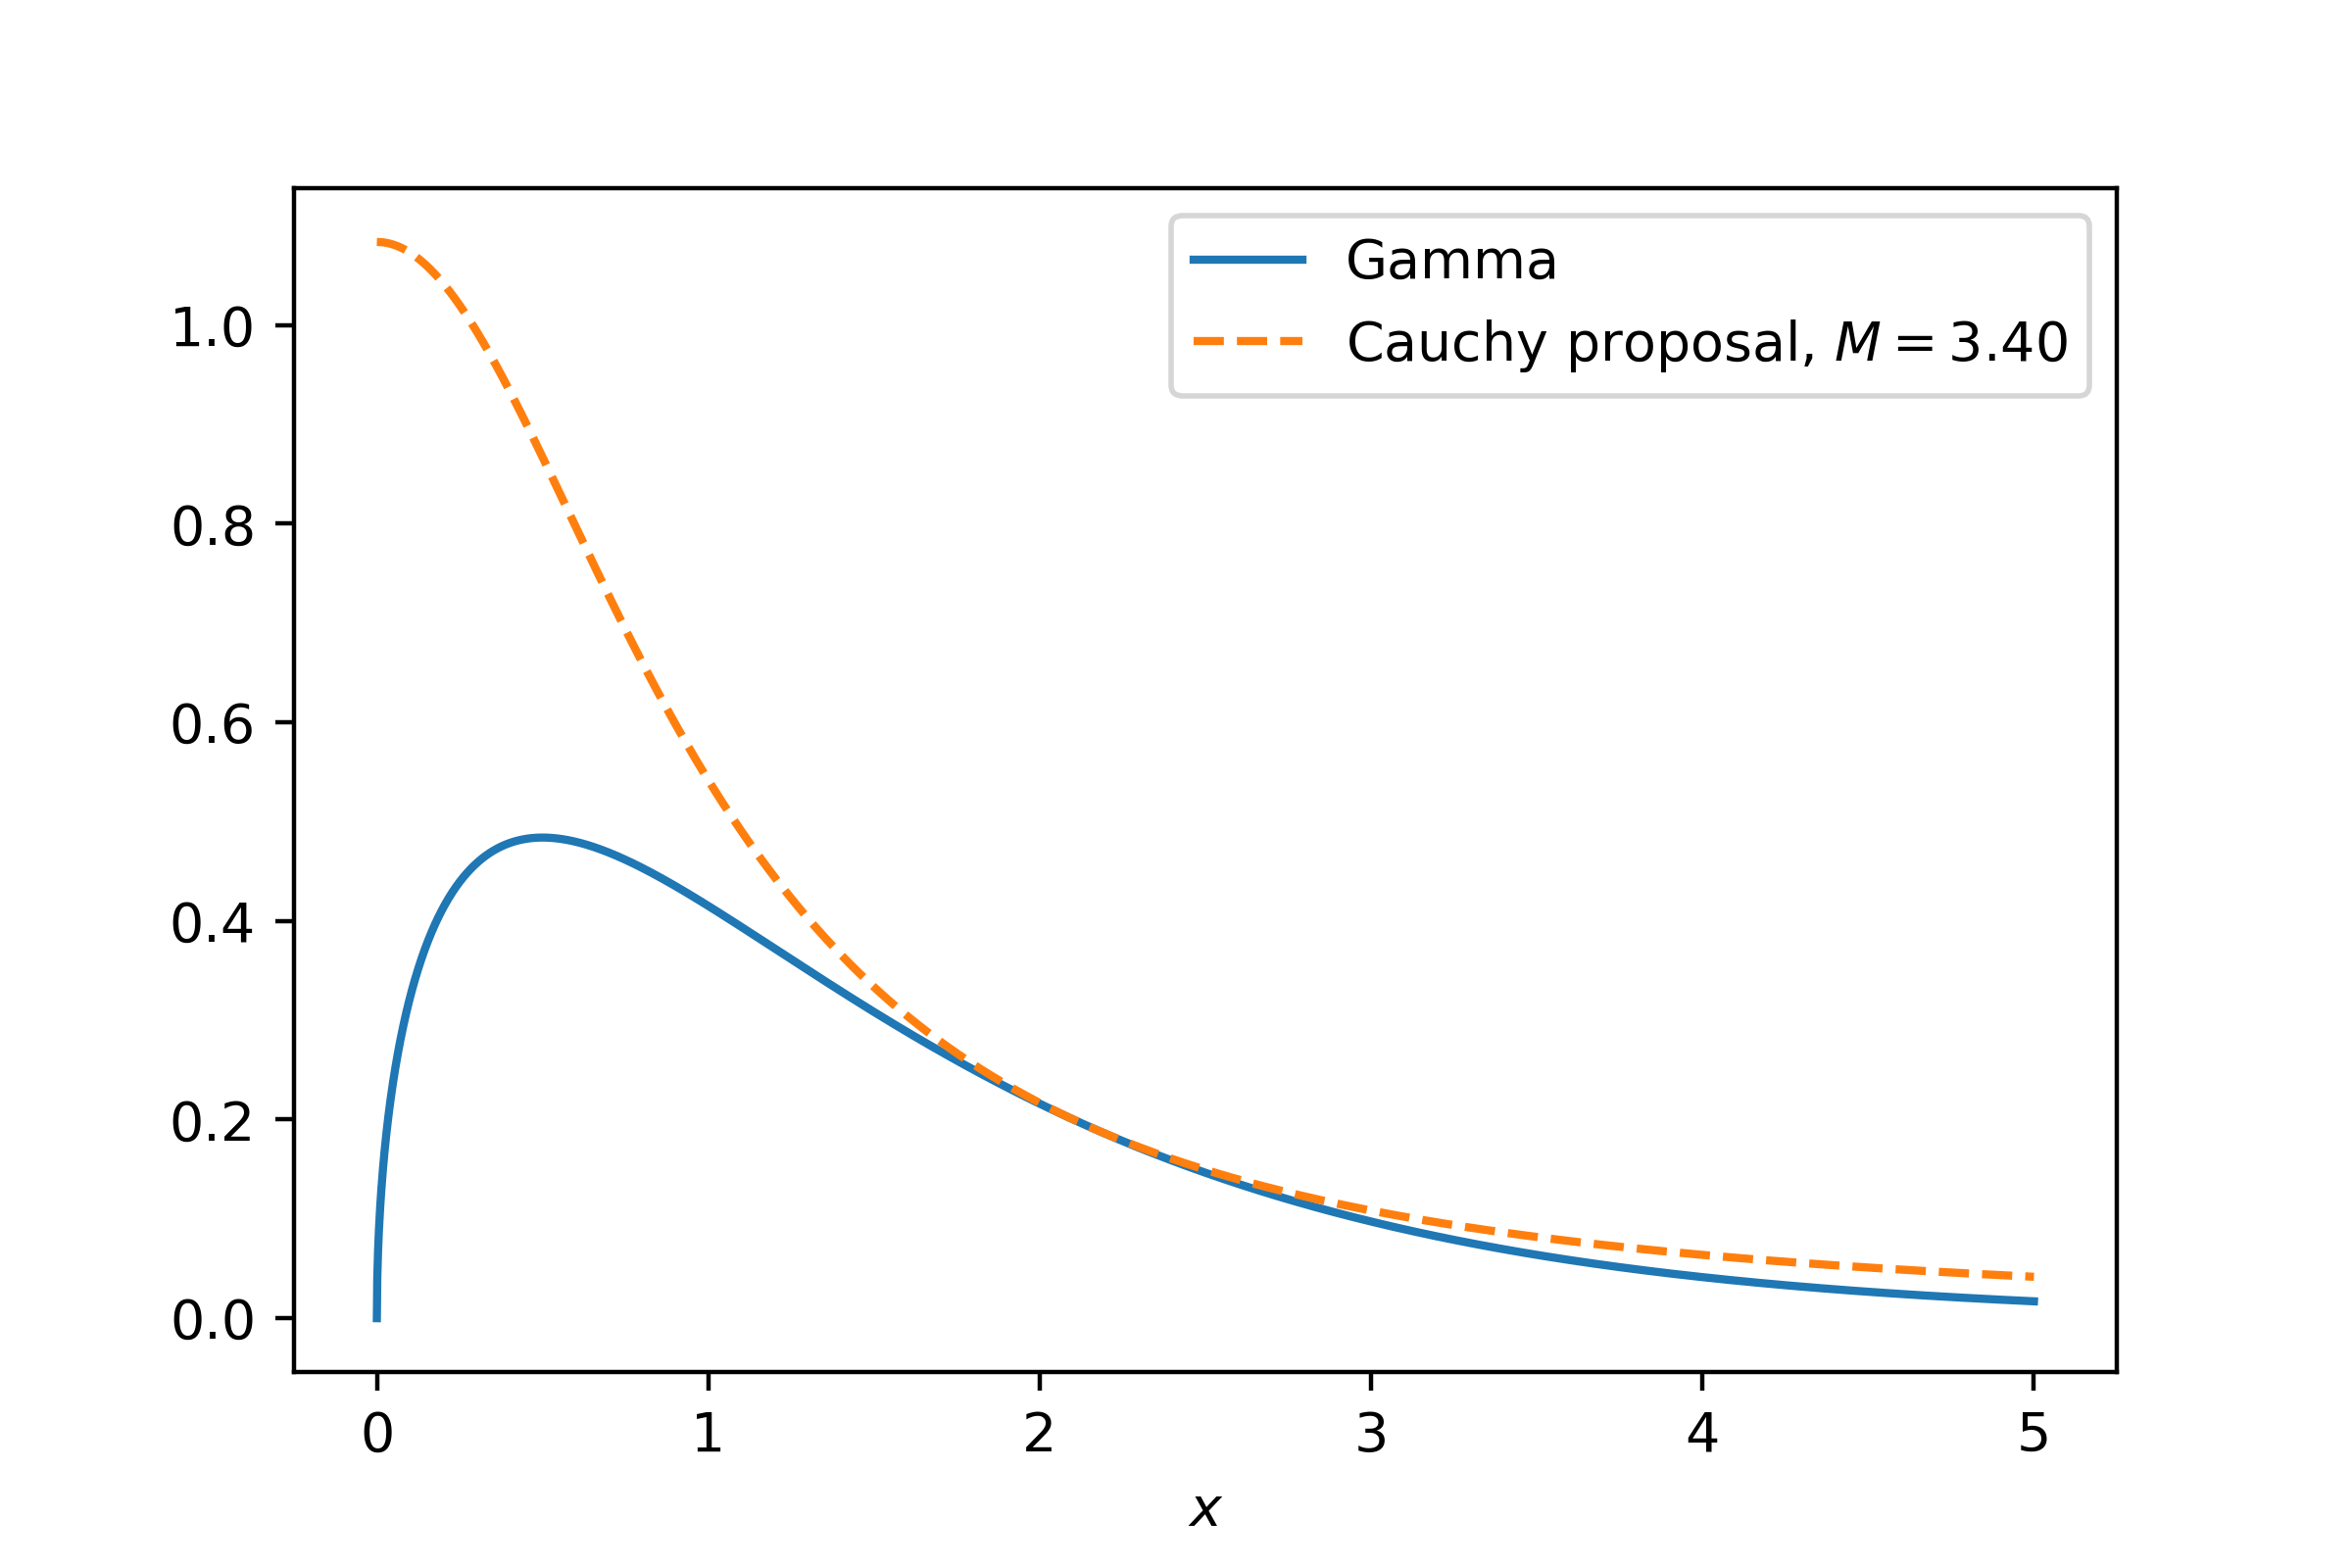
\includegraphics[width=10cm]{rejection-sampling.png}
	\caption{True gamma distribution vs Cauchy proposal with optimal $M$}
	\end{figure}

	The optimal M is given by
	\begin{align*}
		M &= \max \left[
			\frac{ \Ga( x | \alpha, \beta )}{ \mathcal{T}( x | 0, 1, 1 )}
		\right] \\
		&\propto \max\left[
			x ^ { \alpha - 1 } e ^ { -\beta x } \left( 1 + x^2 \right)
		\right].
	\end{align*}
	Deriving the expression inside the max and setting to 0 tells us that
	\[
		M = \left[
			\frac{ \Ga( x^* | \alpha, \beta )}{ \mathcal{T}( x^* | 0, 1, 1 )},
		\right]
	\]
	where $x^*$ is the solution to
	\[
		-\beta x^3 + ( \alpha + 1 ) x^2, -\beta x + \alpha - 1 = 0.
	\]
	I'm not sure which of the roots to pick, but in the demo, there was only one real solution, so I
	just used that one.

	Its pretty easy to see that rejection sampling of a gamma distribution with with a Cauchy
	proposal is fairly inefficient. One reason is that the gamma distribution has no support for
	negative numbers, thus at least half of the samples will be rejected. A better idea might
	be to use a student T distribution with
	$\mu = \frac{ \alpha - 1 }\beta, \sigma^2 = \frac\alpha{ \beta^2 }$
	and $\upsilon=1$. The idea here is to have both distributions have the same mode and scale (note
	that the Cauchy distribution does not have a variance). An even better solution would be to sample
	as in section 23.2 since the gamma cdf has a closed form.

	\exercise
	When the transition dynamics of a model is non-linear, exact inference is intractable, even if
	the observation model is linear. We can see this when looking at the distribution for
	$\mathbf{z}_2$ given $\mathbf{y}_1, \mathbf{y}_2$:
	\[
		p( \mathbf{z}_2| \mathbf{y}_1, \mathbf{y}_2 ) =
		\int p( \mathbf{z}_2 | f(\mathbf{z}_1), \mathbf{y}_2 )
		p( \mathbf{z}_1 | \mathbf{y}_1 ) d\mathbf{z}_1.
	\]
	This is intractable because we have $f$ in the integral, which could be any function.
	However, if we use particle filtering, we no long have to the calculate integral.

	The optimal proposal distribution $q$ is given by equation 23.54. Given the form of our model,
	this is equivalent to having a prior of $\mathcal{N}( f( \mathbf{z}_{t-1} ), \mathbf{Q}_{t-1} )$
	and a likelihood of $\mathcal{N}( \mathbf{H}_t \mathbf{z}_t, \mathbf{R}_t)$. Plugging this into
	equation 4.125, we have
	\begin{align*}
		p( \mathbf{z}_t | \mathbf{z}_{t-1}, \mathbf{y}_{t} )
		&= \mathcal{N}( \mathbf{z}_t | \boldsymbol{\mu}, \boldsymbol{\Sigma} ) \\
		\boldsymbol{\Sigma}^{-1} &= \mathbf{Q}_{t-1}^{-1} + \mathbf{H}_t^T \mathbf{R}_t \mathbf{H} \\
		\boldsymbol{\mu}
		&= \boldsymbol{\Sigma}\left[
		    \mathbf{H}_t^T \mathbf{R}_{t-1}^{-1} \mathbf{y}_t + \mathbf{Q}_{t-1}^{-1}f(\mathbf{z}_{t-1})
		\right].
	\end{align*}
\end{document}

